\section{Experiments}

We evaluate \arena{} along three questions: whether \core{} preserves the probe-level conclusions of the 664-task reservoir, whether the 12-algorithm execution layer is healthy enough for leaderboard use, and whether the resulting leaderboard exposes meaningful algorithmic differences.

\subsection{Experimental setup}

The complete clean evaluation pipeline contains four stages. First, PySR and LLM-SR are run once on the 664-task reservoir, producing $664\times2=1328$ dual-probe runs. Second, 12 algorithms are run once on \candidate{}, producing $200\times12=2400$ calibration runs. Third, the selected \probe{} panel is run on the full reservoir with three seeds, producing $664\times4\times3=7968$ runs. Fourth, all 12 algorithms are run on \core{} with five seeds under a one-hour budget, producing $12\times50\times5=3000$ leaderboard runs.

The 12-method panel is designed to cover the main algorithmic paradigms used in modern SR rather than a single family of GP solvers. It includes classical and modern evolutionary methods (gplearn, PyOperon, PySR, QLattice, RAG-SR), reinforcement-learning and neural-guided methods (DSO, uDSR), tree-search and transformer/planning methods (iMCTS, E2ESR, TPSR), and LLM-assisted equation-discovery systems (LLM-SR, DRSR). \Cref{app:evaluated-baselines} gives the detailed baseline descriptions, including each method's search paradigm, integration contract, and interpretation caveats.

All reported NMSE values use clipped log space:
\[
\log_\mathrm{NMSE}=\mathrm{clip}(\log_{10}(\max(\mathrm{NMSE},10^{-12})),-12,12).
\]
For aggregate leaderboard tables, missing or unevaluable metrics are assigned the worst clipped value before averaging. This prevents invalid outputs from being silently removed.

\subsection{Probe4-Full health and readiness}

The \probe{} full-reservoir stage completed all expected $7968$ runs. Among them, $7616$ runs produced valid outputs. Completion was balanced across the three seeds, each with $2656$ finished runs. Method-level valid rates were $96.9\%$ for DSO, $98.5\%$ for iMCTS, $87.7\%$ for PyOperon, and $99.2\%$ for uDSR. The health gate used for selecting \probe{} is applied during the \candidate{} calibration stage; PyOperon's broader-reservoir valid rate drops below $90\%$, but it remains useful as an evolutionary-GP probe because invalid-prone datasets are explicitly handled by eligibility and limited-quota filters. The postprocessed dataset-level table marks all 664 datasets as complete, with 540 eligible datasets and 124 limited-quota datasets. This makes the Probe4-Full result suitable for \core{} selection.

\subsection{\core{} representativeness}

We compare \core{} against the full 664-task reservoir using the four Probe-4 methods. On the full reservoir, the OOD ranking is
\[
\mathrm{uDSR} \prec \mathrm{iMCTS} \prec \mathrm{DSO} \prec \mathrm{PyOperon},
\]
where lower median log OOD NMSE is better. The same ordering is obtained on \core{}: the paired full-reservoir/\core{} OOD scores are $-5.216/-5.431$ for uDSR, $-4.292/-4.248$ for iMCTS, $-2.305/-2.423$ for DSO, and $-0.410/-0.431$ for PyOperon. The Spearman and Kendall rank correlations between full-reservoir and \core{} Probe-4 aggregate OOD scores are both $1.0$, and all six pairwise method preferences agree.

We also compare \core{} with random and family-stratified random 50-task subsets, plus deterministic alternatives that select by information, metadata diversity, response-space K-medoids, or difficulty balance. \core{} has an aggregate-score MAE of $0.1388$ against the full-reservoir Probe-4 scores, compared with $0.4949$ for random-50 average, $0.5243$ for family-stratified random-50 average, $0.5060$ for metadata-diverse selection, $0.6044$ for response-space K-medoids, $1.0339$ for top-information, and $1.0430$ for difficulty-balanced selection. Thus \core{} reduces aggregate-score error by $72.0$--$86.7\%$ relative to these baselines. Top-information selection has a marginally higher objective score and the highest mean information, but its full-reservoir fidelity is substantially worse. \Cref{tab:core50-ablation-summary} summarizes the curated selector comparison; full definitions are in \cref{app:core50-details}.

\subsection{Leaderboard execution health}

The \core{} leaderboard stage produced all expected 3000 final result files, with no missing or ambiguous artifacts. The status distribution was 2982 \texttt{ok}, 9 \texttt{timed\_out}, and 9 \texttt{no\_valid\_output}. Every algorithm has exactly 250 runs. Ten of the twelve algorithms have 100\% valid-output rate; PyOperon and QLattice have 98.4\% and 98.0\%, respectively.

\begin{table}[t]
\centering
\small
\caption{\textbf{Clean \core{} leaderboard.} Methods are evaluated over 50 datasets and five seeds, ranked by penalized OOD log NMSE (lower is better), and reported with ID log NMSE plus symbolic-fidelity diagnostics. Exact is an SA-style exact-equivalence rate; TreeSim is the TED/NED-style tree-similarity component used by \symf{} (higher is better).}
\label{tab:clean-leaderboard-summary}
\resizebox{\linewidth}{!}{%
\begin{tabular}{rlrrrrrrr}
\toprule
\textbf{Rank} & \textbf{Algorithm} & \textbf{Valid} & \textbf{Metric} & \textbf{ID log} & \textbf{OOD log} & \textbf{\symf{}} & \textbf{Exact \%} & \textbf{TreeSim} \\
\midrule
1 & uDSR & 1.000 & 1.000 & $-6.920$ & $-5.646$ & 36.8 & 24.0 & 0.129 \\
2 & iMCTS & 1.000 & 0.968 & $-4.842$ & $-3.960$ & 41.5 & 30.8 & 0.185 \\
3 & PySR & 1.000 & 0.960 & $-3.848$ & $-3.055$ & 43.6 & 34.0 & 0.242 \\
4 & DSO & 1.000 & 0.972 & $-2.984$ & $-2.458$ & 31.3 & 18.0 & 0.183 \\
5 & DRSR & 1.000 & 1.000 & $-3.396$ & $-2.087$ & 26.8 & 12.0 & 0.098 \\
6 & LLM-SR & 1.000 & 0.992 & $-2.958$ & $-1.420$ & 27.3 & 12.8 & 0.102 \\
7 & gplearn & 1.000 & 1.000 & $-2.013$ & $-1.207$ & 20.0 & 8.0 & 0.085 \\
8 & QLattice & 0.980 & 0.972 & $-2.273$ & $-0.780$ & 17.8 & 4.8 & 0.029 \\
9 & TPSR & 1.000 & 0.996 & $0.200$ & $0.896$ & 15.2 & 0.4 & 0.035 \\
10 & PyOperon & 0.984 & 0.840 & $-0.070$ & $1.079$ & 11.3 & 0.0 & 0.026 \\
11 & E2ESR & 1.000 & 0.800 & $2.049$ & $2.891$ & 12.4 & 0.0 & 0.001 \\
12 & RAG-SR & 1.000 & 0.964 & $3.253$ & $3.788$ & 15.7 & 1.6 & 0.000 \\
\bottomrule
\end{tabular}
}
\end{table}

The expanded metric set follows prior SR benchmark practice: SRBench reports numerical quality together with symbolic-solution and cost indicators; SRSD adds normalized tree-edit distance for expression structure; LLM-SRBench reports ID/OOD NMSE and symbolic accuracy. Accordingly, \cref{tab:clean-leaderboard-summary} keeps the OOD ranking as the primary leaderboard key while exposing whether a method's numerical score is accompanied by symbolic recovery. These results are not intended as the final scientific conclusion of SR as a field. Instead, they demonstrate that SymbolicArena produces a complete, comparable, multi-algorithm evaluation substrate with explicit failure accounting.

\begin{figure}[t]
\centering
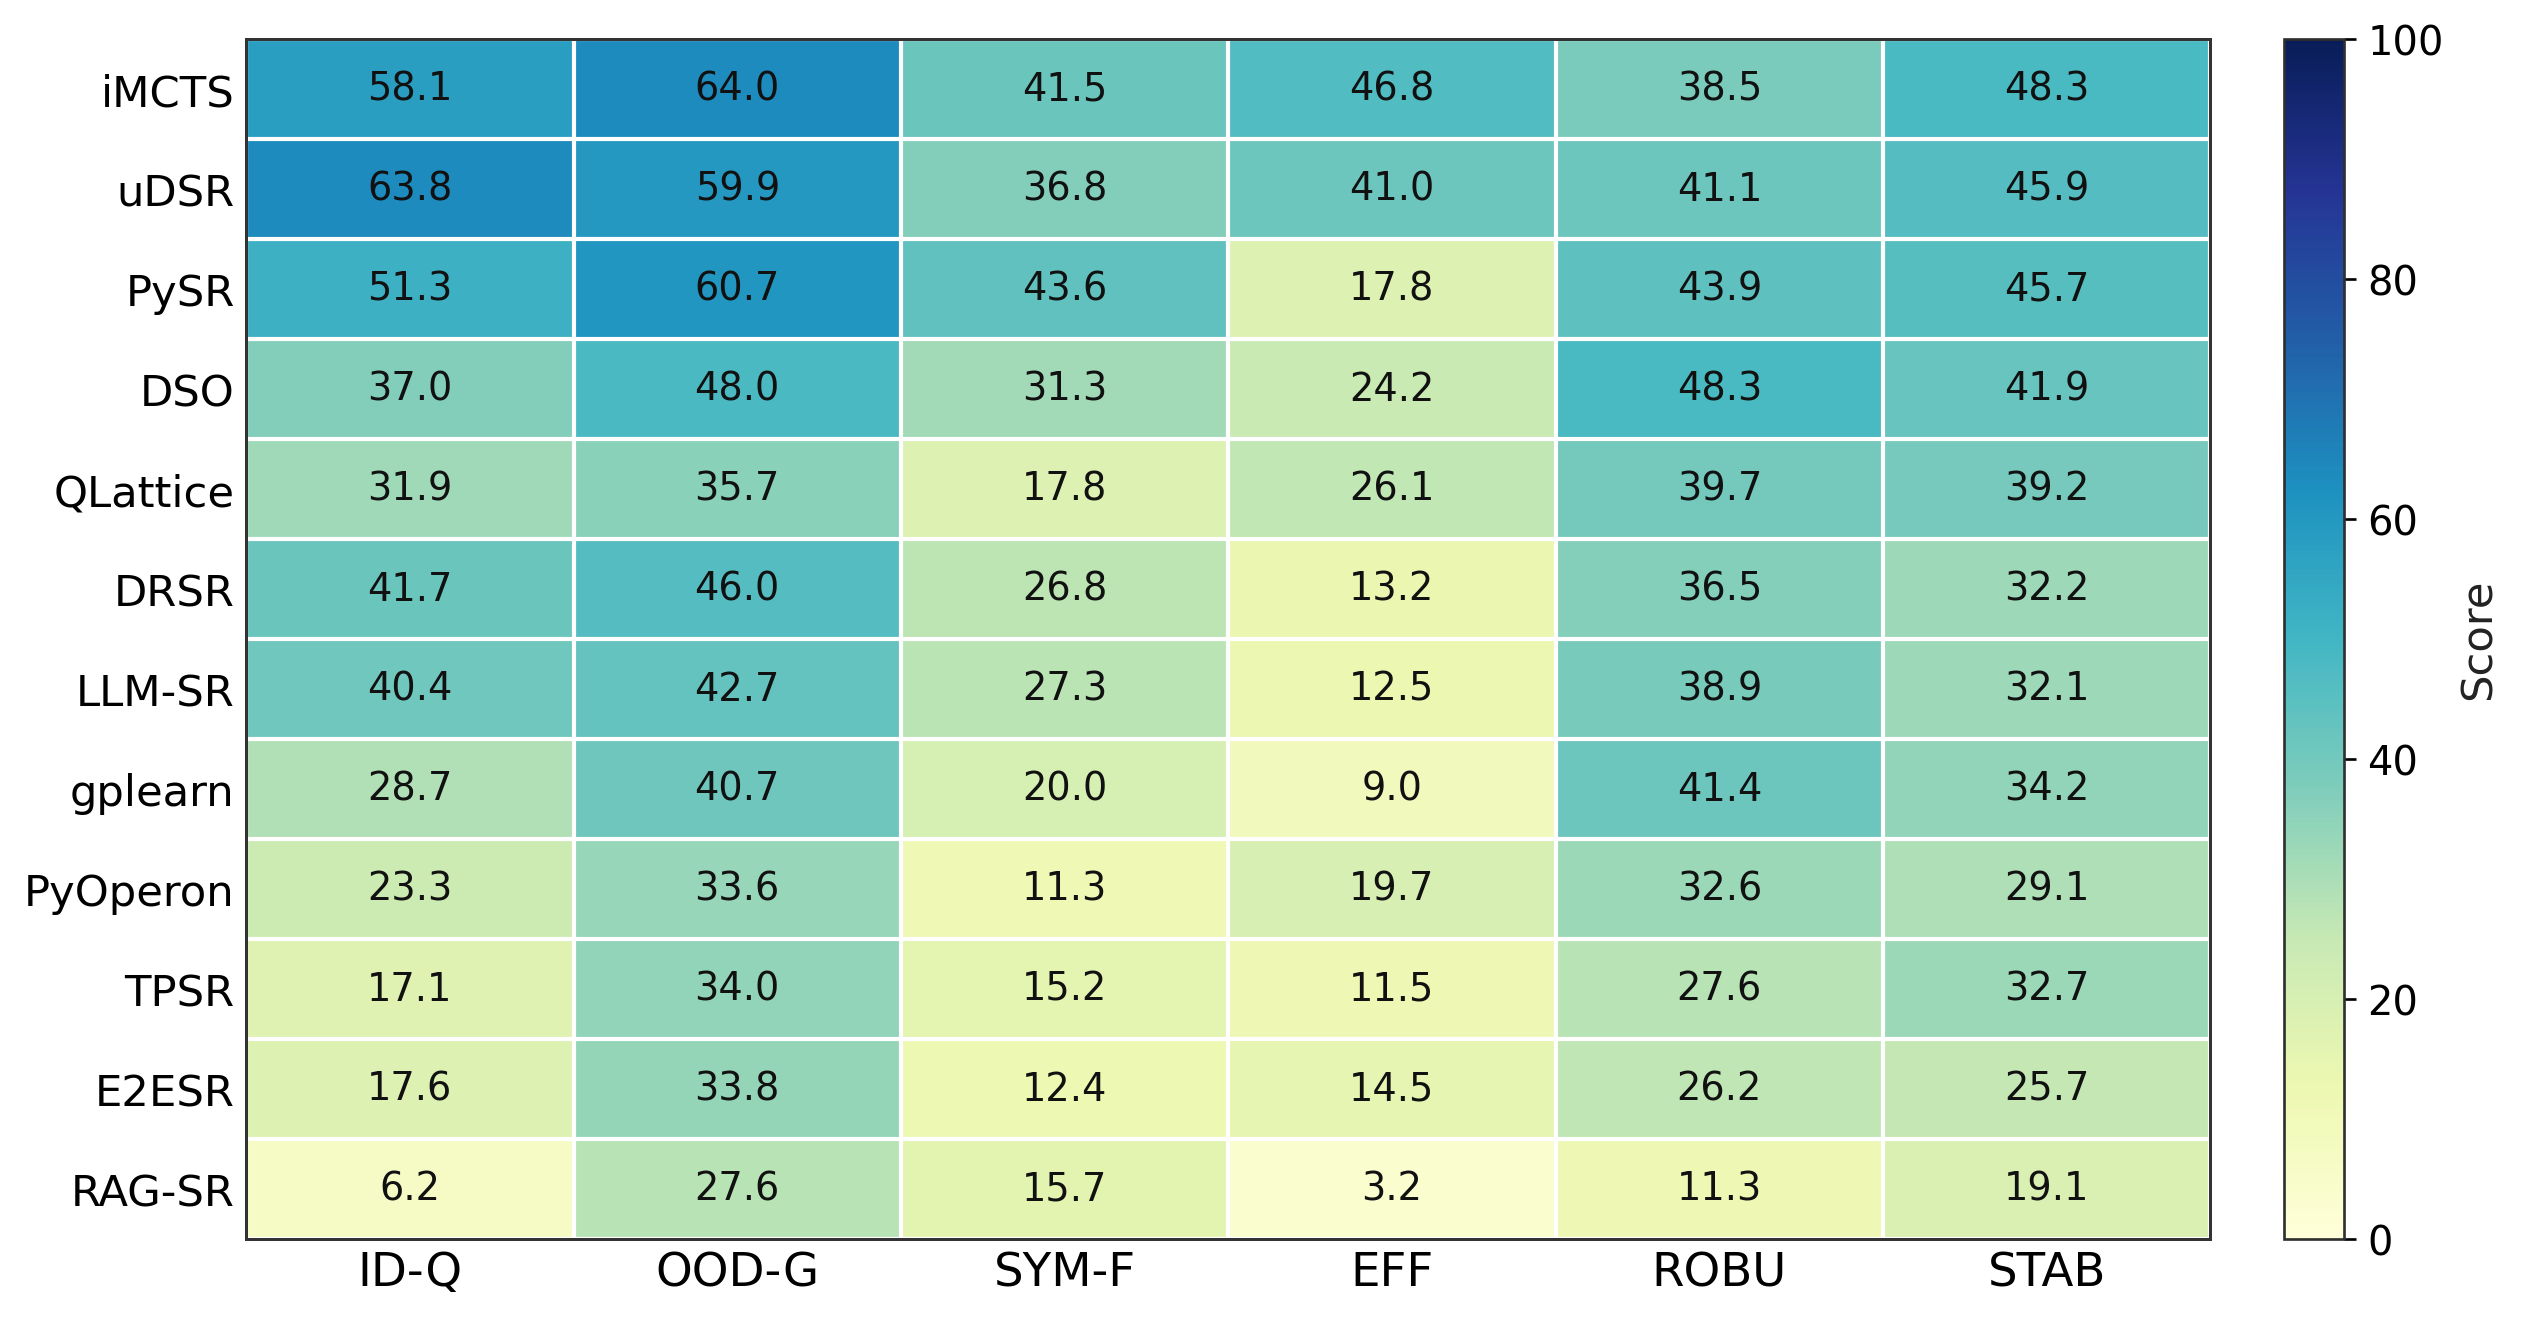
\includegraphics[width=0.90\linewidth]{imgs/Article/figure15_hexagon_heatmap_formal}
\caption{\textbf{Formal clean-track leaderboard heatmap on \core{}.} The heatmap reports \idq{}, \oodg{}, \symf{}, \eff{}, and \stab{}, while \rob{} is marked as a noisy-training extension. It shows that OOD ranking alone does not explain differences in symbolic fidelity, efficiency, and stability.}
\label{fig:hexagon-heatmap}
\end{figure}

\subsection{Dynamic traces and hexagonal evaluation}

The leaderboard protocol records best-so-far expressions every minute, yielding $3000\times60=180000$ search snapshots for the clean \core{} track. Because the trace archive is large, it is packaged as a separate compressed artifact rather than expanded in the paper repository. These traces support time-to-threshold, anytime AUC, complexity-over-time, stagnation, and symbolic-similarity analyses. The clean-track leaderboard reports \idq{}, \oodg{}, \symf{}, \eff{}, and \stab{}; \rob{} is reported only when the shared noisy-training protocol has been completed. The noisy-training robustness curves and heatmap are reported in \cref{app:additional-figures}, because \rob{} is an extension track rather than part of the completed clean-track leaderboard.
